\chapter[SID]{SID}
\label{cap:sid}
\maxwell {Escrever sobre o SID}

\section{Visão Geral} 
O SID está estruturado em duas vertentes, o WEB e o \textit{mobile}, ele foi desenvolvido com o objetivo de oferecer uma aplicação de divulgação que realiza integração com as redes sociais de forma ágil, intuitiva, dinâmica e amigável para os administradores e para os usuários comuns, além de melhorar a efetividade do processo de disseminação das informações referentes ao Campus. Atendendo ao objetivo principal, que é divulgação de informações através de uma plataforma WEB e \textit{mobile}.

Necessitando sempre do uso da rede para realizar atualizações, o SID está dividido em dois módulos e um aplicativo, o primeiro deles é o administrador, onde é possível fazer o gerenciamento completo do conteúdo que será apresentado no segundo módulo chamado cliente, nesse segundo módulo será apresentado as informações que foram cadastradas no módulo administrador, onde então serão propagadas por monitores ou celulares. O aplicativo é um sistema \textit{mobile}, onde o usuário poderá ter acesso a todas as divulgações assim como no módulo cliente, mas com o incremento de troca de mensagens entre professores e alunos através do consumo de uma API fictícia que simula uma sistema de gestão acadêmica. 

A divisão de módulos foi feita para que seja possível atender a arquitetura cliente-servidor, ela mostrou-se necessário para minimizar o processamento dos módulo cliente e do aplicativo que também é considerado um módulo cliente, centralizando o processamento das informações em um sistema mais robusto, ficando a cargo dos clientes exibirem as informações recebidas e realizar pequenos processamentos.

O sistema WEB foi desenvolvido na linguagem PHP, usada para estruturação do projeto, a linguagem JavaScript para realização das requisições de trocas de informações entre os módulos e as linguagens HTML e CSS para desenvolvimento das telas que serão apresentadas no sistema. Usa-se também o Banco de dados PostGreSQL, para armazenamento das informações localmente e que os dados sejam persistentes.

Baseado em desenvolvimento ágil, com metodologia SCRUM, foram definidos sprints semanais, comumente marcada as quartas feiras, para definição das funcionalidades a serem desenvolvidas ou melhoradas. Essa metodologia se torna importante para que o progresso seja acompanhado em cada parte do seu desenvolvimento.

No desenvolvimento, foram usados alguns \textit{framework}, O primeiro deles, usado em conjunto com o PHP, foi o ZEND que tem a finalidade de estruturar o código em modelo, visão e controle. Outro \textit{framework} foi o Doctrine, usado para efetivação da comunicação entre o banco de dados e a orientação a objeto. Foi usado também o Framework7 (F7), em conjunto com o Cordova, para que fosse possível o desenvolvimento do aplicativo mobile. 

Se utilizando dos conceito de UML abordados na Seção \ref{sec:uml}, é  feito a representação dos elementos, demostrando cada artefato do SIDv3, como o diagrama de classe e seus casos de uso.

\section{Modulo Administrador}
Com o uso da arquitetura cliente-servidor, esse módulo fica situado no servidor e é responsável por conceder ao usuário administrador a funcionalidade de gerenciar todas as informações do sistema podendo inserir, alterar, e retirar as divulgações, fazendo todo o gerenciamento das informações que são repassadas ao módulo cliente e \textit{mobile}.

O modelo de casos de uso que representa o módulo é apresentado na figura \ref{fig:casosDeUsoADM}. Ele tem a finalidade de demostrar os principais processos que o administrador pode executar no módulo.

\begin{figure}[H]
\centering
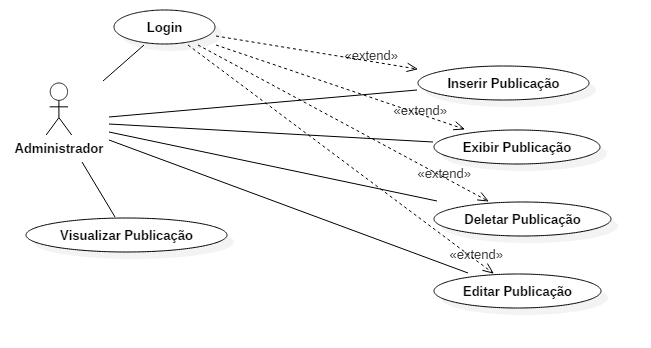
\includegraphics[scale=0.6]{figuras/casosDeUsoADM}
\caption{Casos de uso da ações do módulo administrador}
\label{fig:casosDeUsoADM}
\end{figure}

O acesso ao módulo é restrito, sendo necessário autenticação e para esse fim foi escolhido a ferramenta "\textit{login} com o Facebook", ferramenta que a própria rede social disponibiliza explicada na Seção \ref{sec:autenticacao}. Optou-se pelo uso dela, pois provê maior segurança, sendo baseada em sistemas criptográficos e também por facilitar o processo de recuperação de alguns dados básicos que são necessários para o processo de autenticação com o sistema. O diagrama de sequência que representa o processo de autenticação está representado na figura \ref{fig:sequencialogin}.

\begin{figure}[H]
\centering
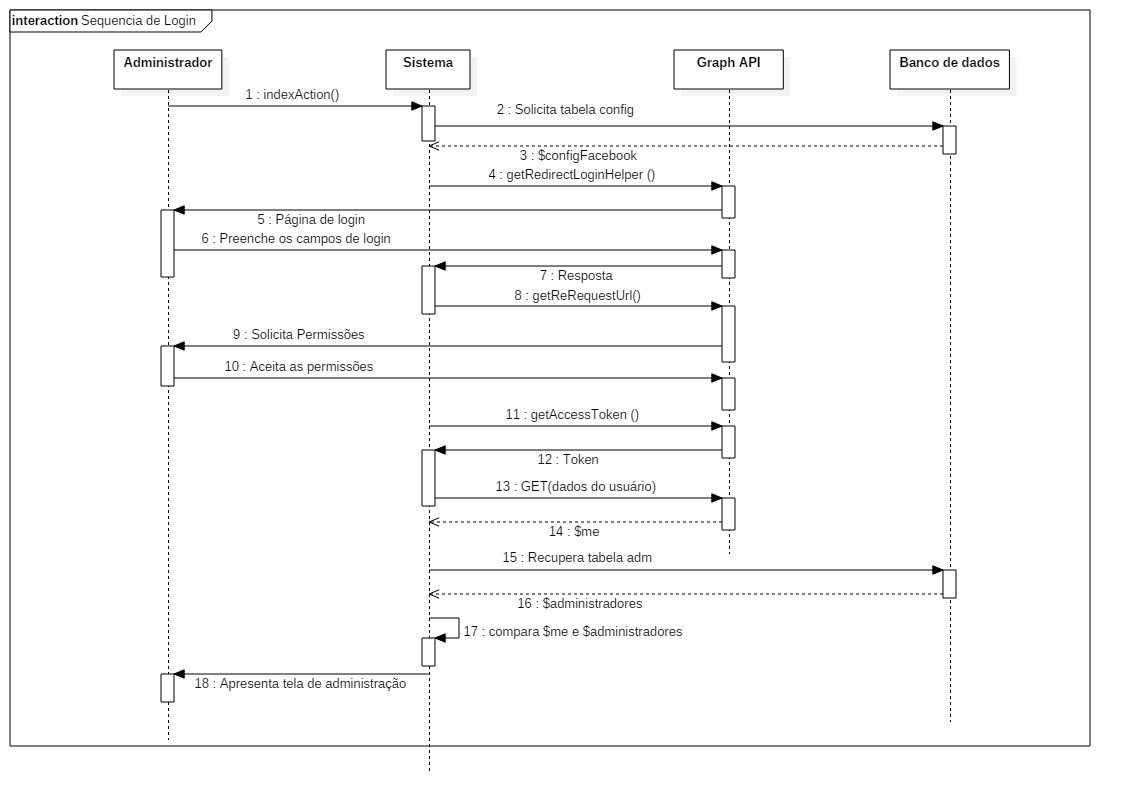
\includegraphics[scale=0.4]{figuras/sequencialogin}
\caption{Sequencia para efetivação de \textit{login}}
\label{fig:sequencialogin}
\end{figure}

A estruturação do banco de dados é composta por três tabelas, sendo mapeadas com as entidades ``config'', ``divulgacao'' e ``adm''. A função da tabela divulgação é armazenar todos os objetos relacionados as divulgações que serão exibidas no cliente e no aplicativo. A tabela adm é usada para armazenar as informações referentes aos administradores do sistema. A tabela config é destinada a armazenar informações únicas para efetivação da comunicação entre aplicativo e Graph API.

\begin{figure}[H]
\centering
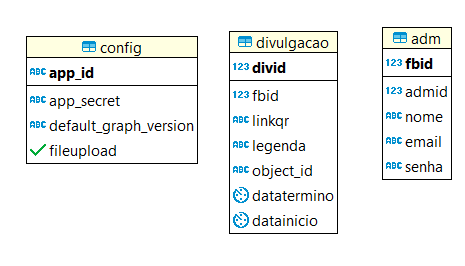
\includegraphics[scale=1]{figuras/entidaderelacionamento}
\caption{Modelo entidade e relacionamento}
\label{fig:casosDeUso}
\end{figure}

A figura \ref{fig:diagramaclasseADM}, mostra a representação e o relacionamento entre as classes disponíveis no módulo. No diagrama de sequência \ref{fig:diagramaclasseADM} é exposto a sequência de uso de cada uma delas. 
\begin{figure}[H]
\centering
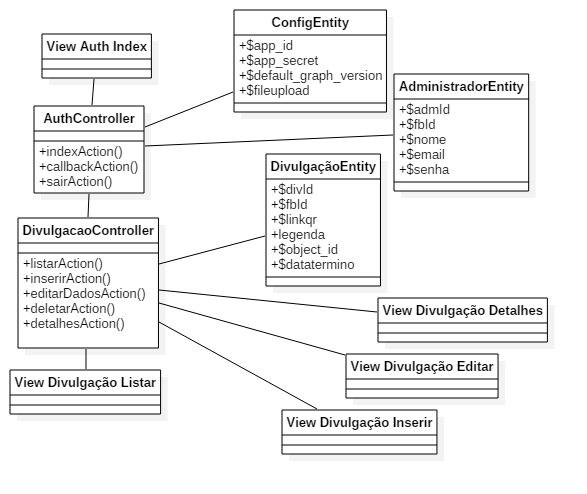
\includegraphics[scale=0.5]{figuras/diagramaclasseADM}
\caption{Diagrama de classe do módulo administrador}
\label{fig:diagramaclasseADM}
\end{figure}

 \begin{figure}[H]
\centering
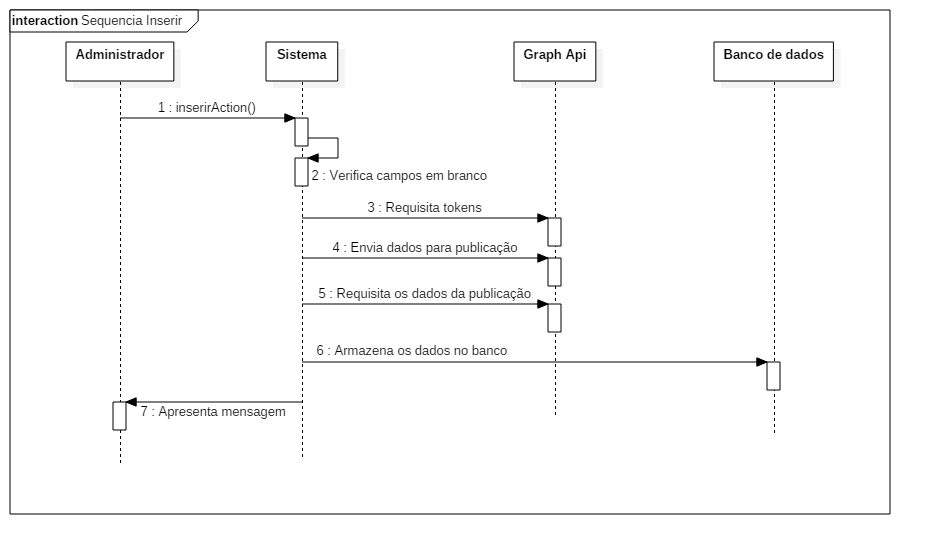
\includegraphics[scale=0.5]{figuras/sequenciainserir}
\caption{Diagrama de sequência para inserção}
\label{fig:sequenciainserir}
\end{figure}

Após a efetivação da autenticação, o usuário poderá ter acesso a todas as funcionalidades disponíveis no sistema, divididas entre as telas de ``inserir'' e ``Home''. A tela de inserir, é usada para criação de uma nova publicação, enquanto a tela Home oferece a opção de listar, detalhar, deletar e editar essa publicações que foram criadas.

A figura \ref{fig:administrador1}, representa a visão do operador da tela de inserir, onde cada elemento da página é enumerado.

\begin{figure}[H]
\centering
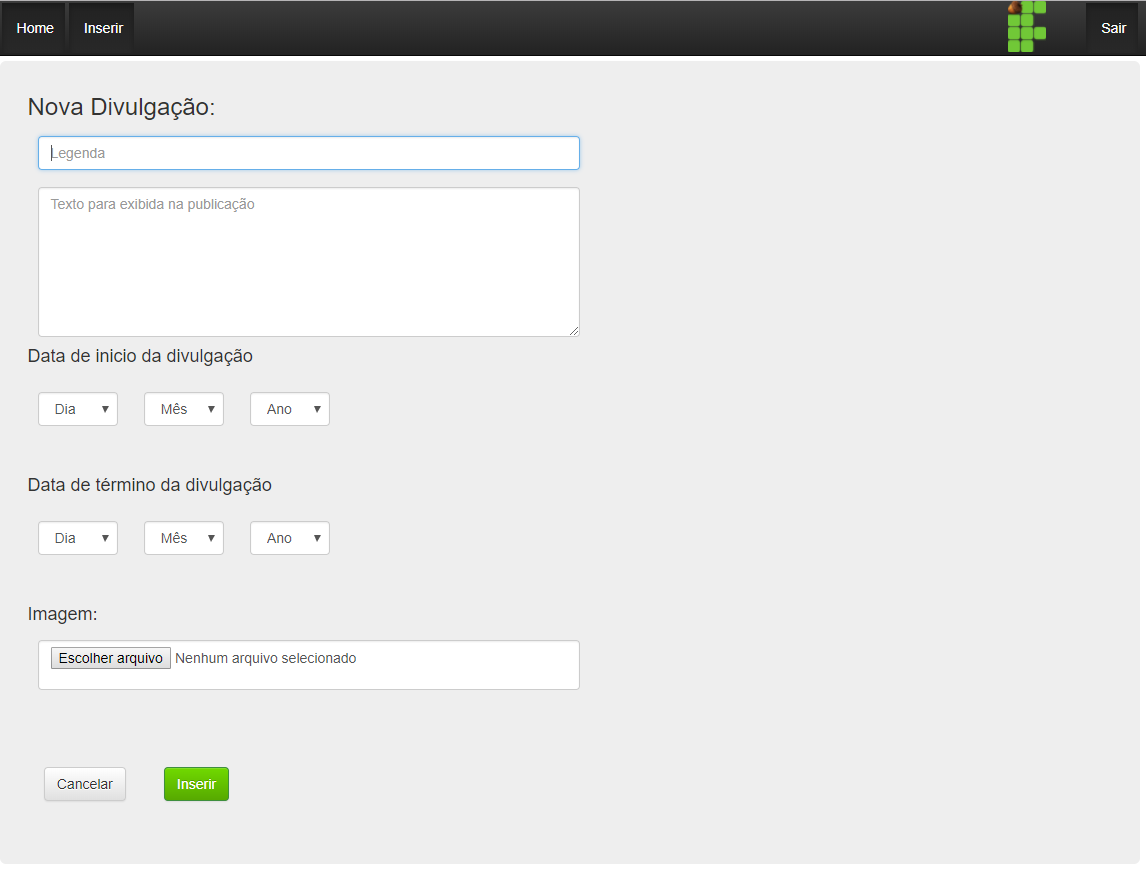
\includegraphics[scale=0.5]{figuras/administrador1}
\caption{Página de inserção do módulo administrador.}
\label{fig:administrador1}
\end{figure}

Os elementos presentes na tela de inserir são listados abaixo, juntamente com suas funcionalidades: 

\begin{enumerate}
   \item Legenda: É um campo de texto destinado a informação a ser repassada de forma sucinta e clara ao usuário final por intermédio cliente ou mobile. 
   \item Texto: É todo o texto que será enviado ao Facebook, contendo informações como descrição da publicação, data e horário da realização e um possível \textit{link} para acesso a mais informações. 
   \item Data de Início: É a data inicial em que a publicação começará a ser exibida no cliente e no mobile.
   \item Data de Término: É a data final em que a publicação deixará de ser exibida no cliente e no mobile.
   \item Imagem: Será a imagem enviada para o Facebook, para o cliente e para o mobile. Essa imagem pode ser um \textit{banner} de apresentação de um evento, por exemplo.
 \end{enumerate}

Todos os campos são de preenchimento obrigatório. O campo 5 é repassado para a API como parâmetro \textit{source}, já o campo 2 é repassado como parâmetro \textit{messagem}, os outros campos são enviados somente para o banco de dados.

Se durante o envio alguma das transações não forem efetivadas, será retornado a mensagem de erro na tela, assim como retornará a mensagem de sucesso, caso não ocorra nenhum erro.

O texto do campo 1 poderá conter letras ou números, entretanto possui a limitação máxima de 80 caracteres, isso é necessário para facilitar a leitura do usuário ao texto que será inserido, pois ele será armazenado no banco de dados e recuperado no módulo cliente para exibição.

Os outros campos não possuem limitação de caracteres, entretanto os campos 3, 4 e 5 possuem restrição de tipo de entrada, onde os campos 3 e 4 obrigatoriamente será um número inteiro e o campo 5, será um arquivo de imagem do tipo JPEG, JPG, GIF ou PNG.

Os campos 3 e 4 são botões do tipo dropdown, sendo necessário selecionar um dos valores que aparecem em cada um dos campos. Os possíveis valores para o campo ``dia'' vão de 1 a 31, os valores do campo ``mês'' vão de 1 a 12, enquanto os valores do campo ``ano'' irão do ano atual a dois anos seguintes.

A página "Home" é responsável por listar todas as publicações criadas, a visão do usuário será a mesma que representada na figura \ref{fig:administrador2}. As funcionalidade de cada elemento da página é descrito logo abaixo. Essa é a página inicial do sistema, nela é possível ter acesso a página de inserir, listar, detalhar e ao botão excluir.

\begin{figure}[H]
\centering
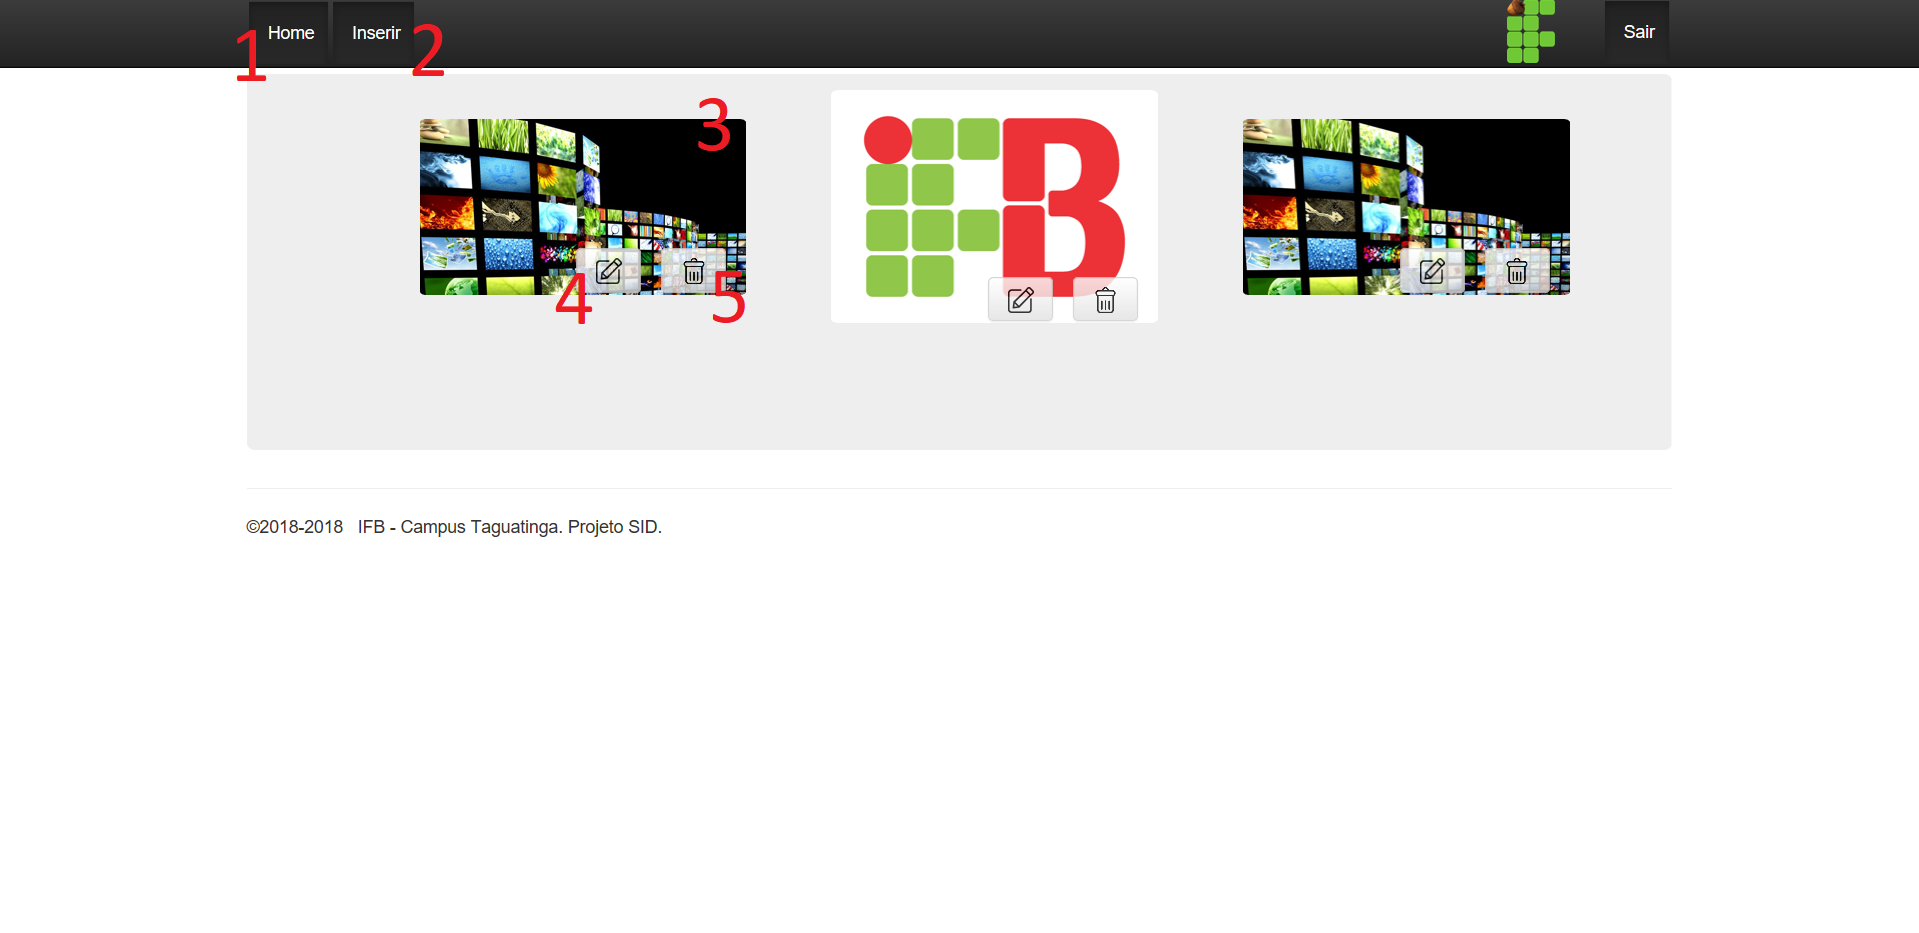
\includegraphics[scale=0.4]{figuras/administrador2}
\caption{Página de listagem  do módulo administrador.}
\label{fig:administrador2}
\end{figure}

\begin{enumerate}
   \item Home: 
   \item Inserir: 
   \item Detalhes: 
   \item Editar: 
   \item Excluir: 
 \end{enumerate}

\subsection{Módulo API}
Fazendo parte do módulo administrador, esse módulo possui a finalidade de recuperar os dados das publicações realizadas pelo administrador no Facebook, estrutura-los de forma que atenda a arquitetura REST e realizar o controle de alguns dados. Isso é necessário para que o módulo cliente e o aplicativo possam realizar requisições de solicitação ou envio de dados.

O controle de dados realizado pelo módulo API é necessário para que conteúdos como comentários inadequados não sejam exibidos. Para esse controle é efetuado uma varredura de todos os usuários que curtiram cada comentários da publicação, caso seja encontrado a curtida de um dos administrador cadastrados no banco de dados o comentário é aprovado para ser exibido.

Além disso, as requisições para esse módulo devem seguir uma sintaxe de acordo com os dados desejados. Como mostra o exemplo \ref{lst:bd}, onde é requisitado as informações das publicações presentes no banco.

\begin{lstlisting}[caption={Requisitando dados para divulgação},label={lst:bd}]
	http://{IP DO SERVIDOR}:{PORTA}/bd
\end{lstlisting}

A resposta para a solicitação \ref{lst:bd} é uma estrutura de dados do tipo JSON contendo o conteúdo apresentado no exemplo \ref{lst:retornobd}. O uso de cada um dos itens será explicado na Seção \ref{sec:cliente}.

\begin{lstlisting}[caption={Retorno da requisição \ref{lst:bd}},label={lst:retornobd}]
	COLOCAR RETORNO
\end{lstlisting}

Este módulo tem a função de em conjunto com banco de dados, realizar a simulação de um sistema de gestão acadêmico, sendo possível consultar alguns dados através de requisições. Os dados que podem ser recuperados, variam de acordo com a sintaxe utilizada.

É possível requisitar diversos dados distintos ou todos eles juntos. 
No exemplo \ref{lst:todos} é feito a requisição de todos os dados armazenados, que retornará um JSON de diversas posições, onde cada posição representa um ??.
\begin{lstlisting}[caption={Requisitar todos os dados},label={lst:todos}]
	http://{IP DO SERVIDOR}/mobile
\end{lstlisting}

\begin{lstlisting}[caption={Retorno da requisição \ref{lst:todos}},label={lst:retornotodos}]
	Exemplo de retorno
\end{lstlisting}

A inclusão de um novo parâmetro na requisição \ref{lst:todos} torna a busca mais específica. Por exemplo, pode ser usado "/professores", "/alunos", "/turmas" ou "/mensagens", isso retornará um JSON contendo somente a lista com os dados solicitados. No exemplo \ref{lst:professores}, o retorno será uma lista com os dados de todos os professores cadastrados como mostra o exemplo \ref{lst:retornoprofessores}.

\begin{lstlisting}[caption={Requisitar lista de dados especifica},label={lst:professores}]
	http://{IP DO SERVIDOR}/mobile/professores/
\end{lstlisting}

\begin{lstlisting}[caption={Retorno da requisição \ref{lst:bd}},label={lst:retornoprofessores}]
	RETORNO
\end{lstlisting}

O diagrama de classe que representa esse módulo é descrito na figura \ref{fig:diagramaclasseAPI}. Cada uma das classes é usada para uma determinada requisição.
\begin{figure}[H]
\centering
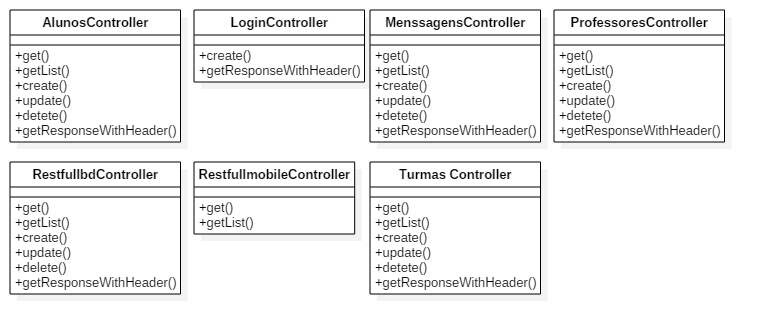
\includegraphics[scale=0.5]{figuras/diagramaclasseAPI}
\caption{Diagrama de classe do módulo API}
\label{fig:diagramaclasseAPI}
\end{figure}

\section{Módulo Cliente}
\label{sec:cliente}
O modulo cliente tem a função de apresentar as divulgações de maneira atrativa, intuitiva e dinâmica para o usuário. O seu caso de uso é apresentado na figura \ref{fig:casosDeUsoCliente}. A estrutura e organização do que será apresentado, está disposto na figura \ref{fig:cliente1} e o seu diagrama de classe é apresentado na figura \ref{fig:diagramaclasseCLIENTE}.

\begin{figure}[H]
\centering
\includegraphics[scale=0.6]{figuras/casosDeUsoCliente}
\caption{Casos de uso da ações do módulo cliente}
\label{fig:casosDeUsoCliente}
\end{figure} 

\begin{figure}[H]
\centering
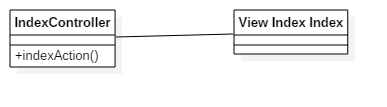
\includegraphics[scale=0.4]{figuras/diagramaclasseCLIENTE}
\caption{Diagrama de classe do módulo cliente}
\label{fig:diagramaclasseCLIENTE}
\end{figure}

Os elementos que compõe a página que será apresentada, são divididos em cinco itens, que estão descritos abaixo.

\begin{enumerate}
   \item Imagem: O conteúdo, poderá ser apresentado como uma imagem estática ou como GIF (imagem com animação), não oferecendo suporte a vídeos, até o momento, mas que poderá ser implementado em versões futuras. 
   \item Legenda: A legenda é apresentada em movimento linear da direita para a esquerda, possibilitando a leitura de forma dinâmica de toda a frase.
   \item QR Code: Imagem, que por meio de um aplicativo celular, possibilita a leitura que contém o \textit{link} de acesso a publicação publicada na rede social Facebook.
   \item Horário: Relógio que apresentará a data e hora atual.  
   \item Comentários: Espaço que será apresentado comentários publicados e devidamente moderados.
 \end{enumerate}
  
\begin{figure}[H]
\centering
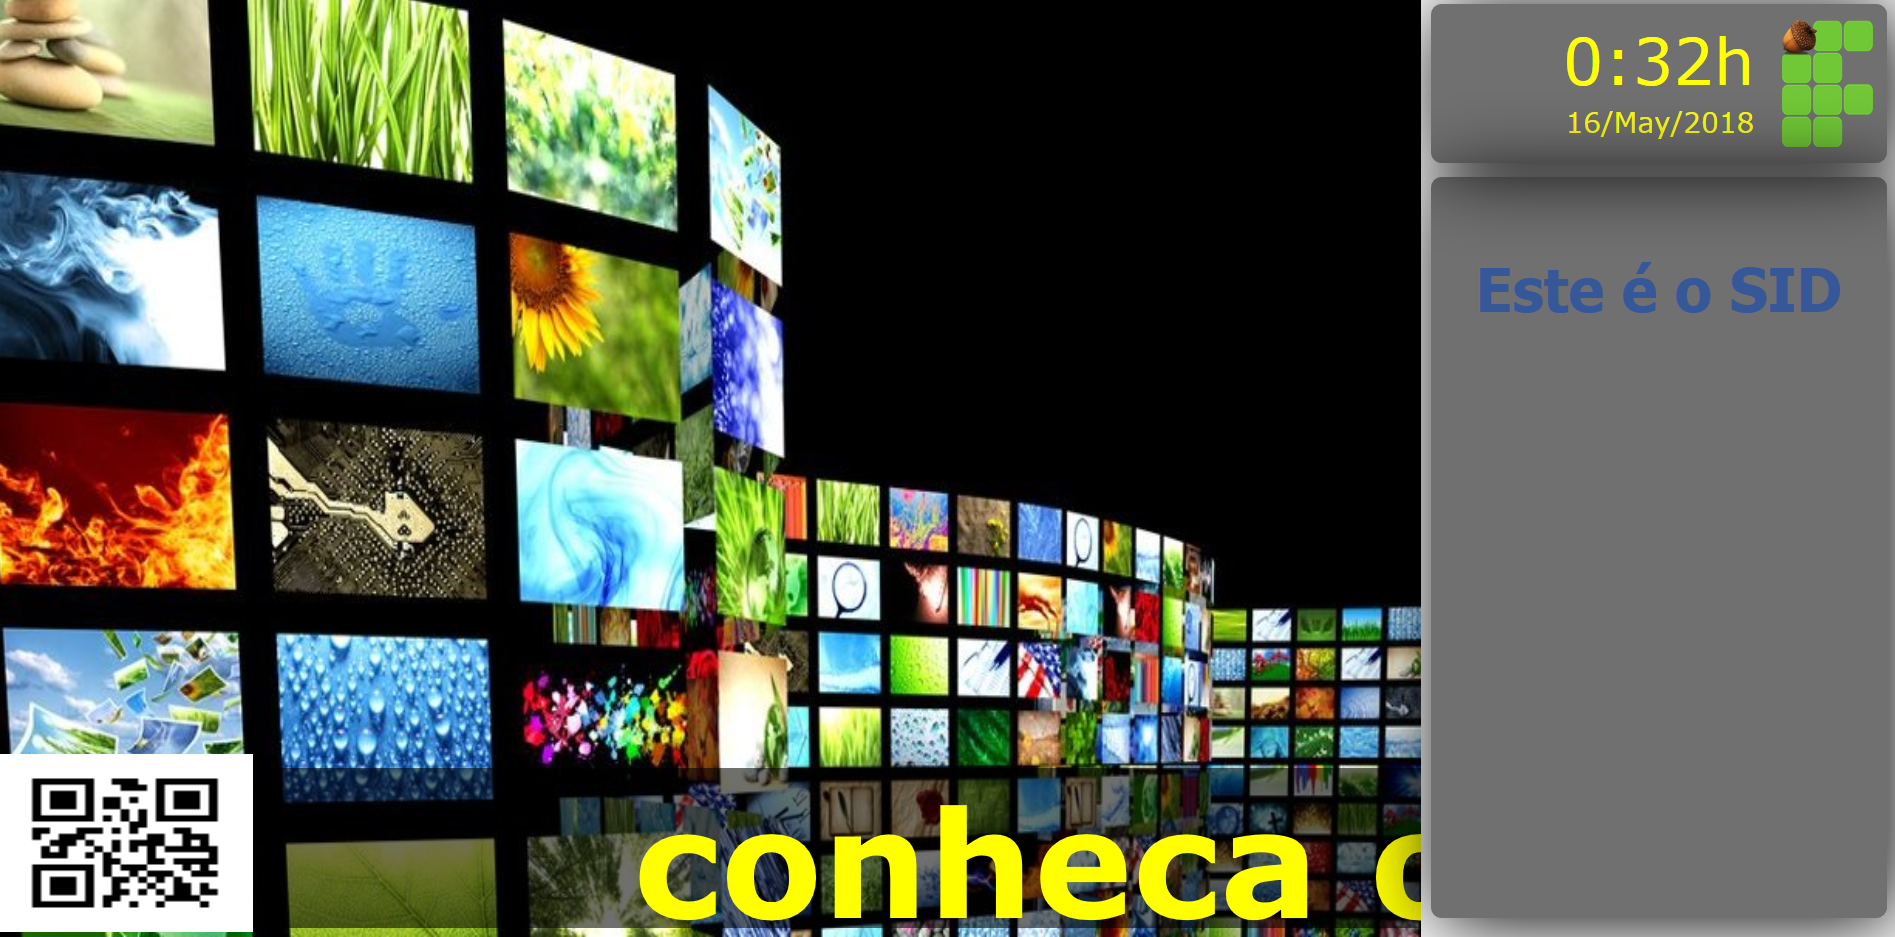
\includegraphics[scale=0.3]{figuras/cliente1}
\caption{Página do cliente}
\label{fig:cliente1}
\end{figure}

Consumindo uma API REST através de requisições do tipo GET, o módulo cliente receberá como resposta um JSON, contendo o número de posições equivalentes ao número de publicações válidas. Cada posição desse JSON terá três variáveis, são elas: 'bd','comentarios' e 'imagem'. 

\begin{lstlisting}[caption={Solicitação de dados ao servidor},label={lst:solicitacaoServidor}]
EXEMPLO DE SOLICITACAO
\end{lstlisting}

A 'bd', contém uma \textit{array} de duas posições, contendo 2 \textit{string}, sendo elas o legenda e link, esses dados foram armazenados pelo servidor no banco de dados, na criação da publicação. A 'comentarios' é um array de \textit{string} que pode possuir zero ou mais itens, cada item representa um comentário na publicação, onde cada item possui a data da criação, quem fez, a mensagem, a foto e o id do comentário. Já a 'imagem' é uma \textit{string} de é um arquivo codificado em base64, que será descodificado pelo módulo.

\begin{lstlisting}[caption={Resposta do servidor \ref{lst:solicitacaoServidor}},label={lst:RespostaServidor}]
EXEMPLO DE RESPOSTA
\end{lstlisting}

O conteúdo recuperado da variável 'bd', será apresentado nos itens 2 e 3, respectivamente. Já o conteúdo recuperado da variável 'comentarios' será apresentado no item 5. Enquanto os da variável 'imagem', será descriptografado e apresentado em forma de imagem no item 1.

O campo 5 irá apresentar 5 elementos recuperados na variável 'comentarios'. Esses elementos serão: a imagem de perfil, o nome, o comentário, a data e a hora da publicação do comentário pelo usuário. Antes da apresentação das informações de comentários, é escolhido um número randômico que representará a posição do array do comentário que será apresentado.

\section{Aplicativo Mobile}
O \textit{mobile} apresentará na tela inicial os mesmos dados que são apresentados no módulo cliente, com a inclusão da funcionalidade de troca de mensagens entre professores e alunos que possuam um login e senha cadastrados.

Os casos de uso do aplicativo é demostrado na figura \ref{fig:casosdeusomobile}, enquanto o modelo entidade e relacionamento é apresentado na figura \ref{fig:entidaderelacionamentomobile}.
\begin{figure}[H]
\centering
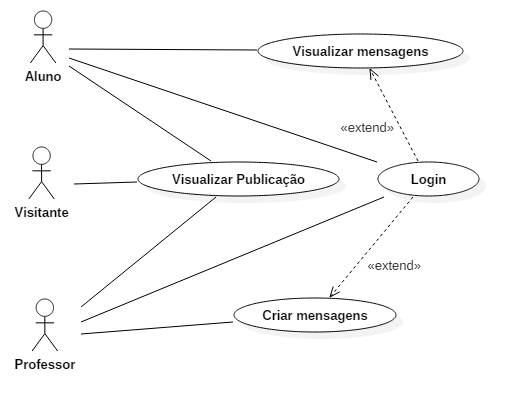
\includegraphics[scale=0.4]{figuras/CasosDeUsoMobile}
\caption{Modelo entidade e relacionamento}
\label{fig:casosdeusomobile}
\end{figure}

\begin{figure}[H]
\centering
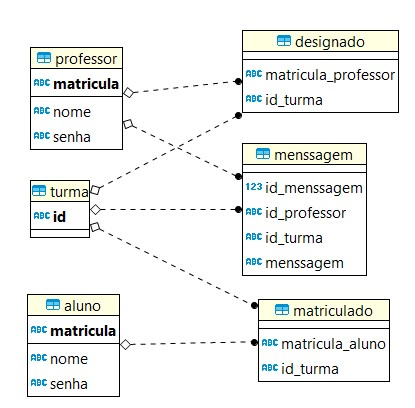
\includegraphics[scale=0.8]{figuras/entidaderelacionamentomobile}
\caption{Modelo entidade e relacionamento}
\label{fig:entidaderelacionamentomobile}
\end{figure}

O aplicativo terá três telas distintas que será a tela inicial, a tela do aluno e a tela do professor. Cada uma terá uma funcionalidade específica, onde a tela de professor e aluno serão restritas a usuários logados e a tela inicial será pública.

A tela inicial será apresentada como na figura \ref{fig:mobile1}, exibindo o nome do SID e o botão de login na parte superior e as publicações válidas, que foram requisitadas do servidor, no restante da tela.
\begin{figure}[H]
\centering
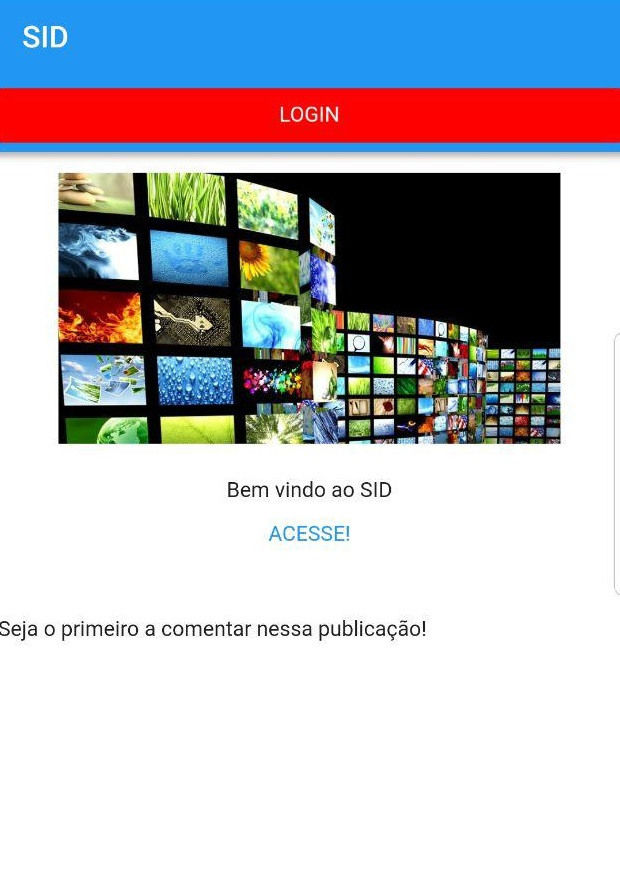
\includegraphics[scale=0.45]{figuras/mobile1}
\caption{Página de inserção no módulo administrador.}
\label{fig:mobile1}
\end{figure}

A tela do aluno será apresentada como na figura \ref{fig:mobile2}, após o login, será apresentado ao aluno todas as mensagens que o aluno possui em ordem cronológica da mais nova para a mais antiga. Os campos apresentados são o de professor, turma e mensagem separando cada item por blocos.

\begin{figure}[H]
\centering
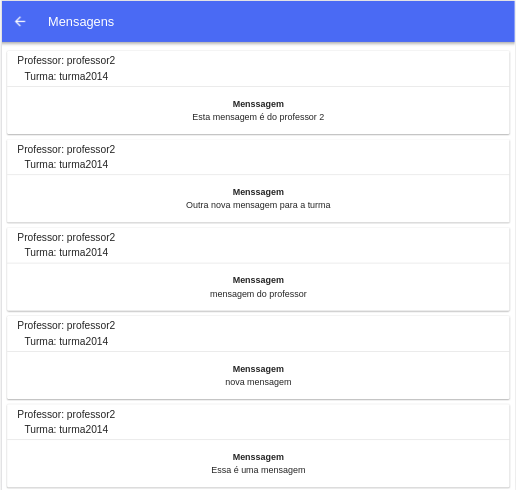
\includegraphics[scale=0.4]{figuras/mobile3}
\caption{Página do Aluno.}
\label{fig:mobile2}
\end{figure}

Já a tela do professor será apresentada conforme a figura \ref{fig:mobile3}, após o login, será apresentado ao professor a matricula dele, a lista de turmas que ele leciona e uma caixa de texto que o professor usará para digitar a mensagem.

\begin{figure}[H]
\centering
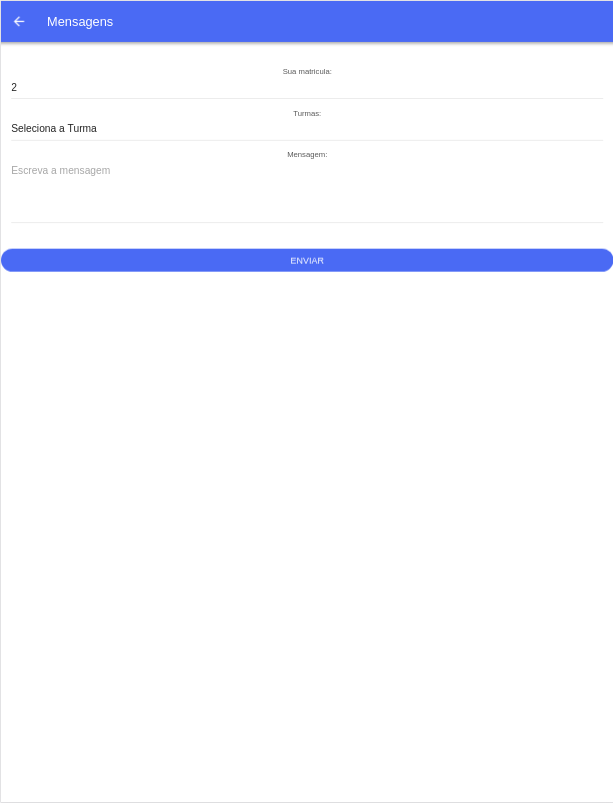
\includegraphics[scale=0.5]{figuras/mobile2}
\caption{Página do professor.}
\label{fig:mobile3}
\end{figure}

\section{Integração}
\subsection{\textit{login}, \textit{token} de acesso e permissões}
Para autenticação e efetivação de todas as requisições feitas pelo módulo administrador para o Facebook é necessário que um \textit{login} seja feito. Para isso, é utilizado a ferramenta de \textit{login} do Facebook que é disponibilizada pela rede social.

A ferramenta de \textit{login} do Facebook que é disponibilizada pela rede social, oferece um botão que pode ser colocado na página, esse botão tem a finalidade de iniciar o processo de login. Após ser clicado é efetuado o processo de login conforme segue padrão estabelecido solicitando as credenciais cadastradas na rede social, com isso é feito a requisição com as permissões necessárias conforme exemplo \ref{lst:solicitacaologin}.

No processo de \textit{login} são solicitados algumas permissões, como as permissões “email”, “manage\underline{{ }}pages” e “publish\underline{{ }}pages”, sendo obrigatório o acete para acesso ao sistema. Usadas respectivamente para que seja possível a identificação do usuário do SID, para recuperar as permissões de acesso a página e a última para permitir que aplicativos publiquem na página \cite{facebook2018a}.

O uso de um usuário vinculado a rede social se torna necessário pois existe a necessidade da página apresentar qual o perfil está realizando a ação, além da necessidade de moderação dos comentários que serão exibidos.  Além disso, para efetivação de todas as requisições feitas pelo módulo administrador para o Facebook, seja ela para requisitar informações das publicações ou realizar uma nova publicação, é usando o \textit{token} de acesso de usuário, que é obtido no processo de login, conforme exemplo \ref{lst:tokenUsuario}.

Entretanto, o uso de um usuário cadastrado na rede social não é o único requisito par acesso ao sistema. Para o acesso é necessário também um usuário administrador, cadastrado no banco de dados do SID. Essa ação é necessária para que somente usuários autorizados possam realizar alteração na página usando o sistema.

Após o login, algumas informações usadas são guardadas na sessão do usuário, para usos posteriores. Entretanto, todo o processo de armazenamento de informações, envios ao Facebook e retornos de solicitações não devem ser visíveis ao usuário. 

\subsection{Publicar}
Todas as publicações realizadas no Facebook usando o SID são feitas ao nó ``/photo'', onde a cada nova publicação será gerado um ID para ela e terá a mesma estrutura de uma imagem postada por um usuário convencional desta rede social.

Na criação de uma nova publicação, usando o SID, são passados para a Graph API dois parâmetros para inserção através do método POST, conforme exemplo \ref{lst:requisicao9}, o primeiro deles é “message”, onde será passado o texto que será exibido na publicação e o outro é “source”, onde será passado a imagem para ser exibida juntamente com o texto. Para envio de imagem para a rede social, é necessário passar na imagem como parâmetro o método “fileToUpload” conforme exemplo \ref{lst:appesdk}. 

Alguns dos elementos que são solicitados pela aplicação na criação de uma nova publicação, são omitidos no envio para o Facebook, pois esses dados serão usados apenas para serem armazenados no banco para uso do módulo cliente. Os elementos omitidos são os campos data de início, a data de termino e a legenda. 

A Figura \ref{fig:imgfacebook1} apresenta como ficará uma publicação no Facebook após o uso do SID para criação da mesma. Nela é apresentado informações como quem realizou a publicação, o texto e a imagem que foram informados durante a criação da divulgação pelo SID.

\begin{figure}[H]
\centering
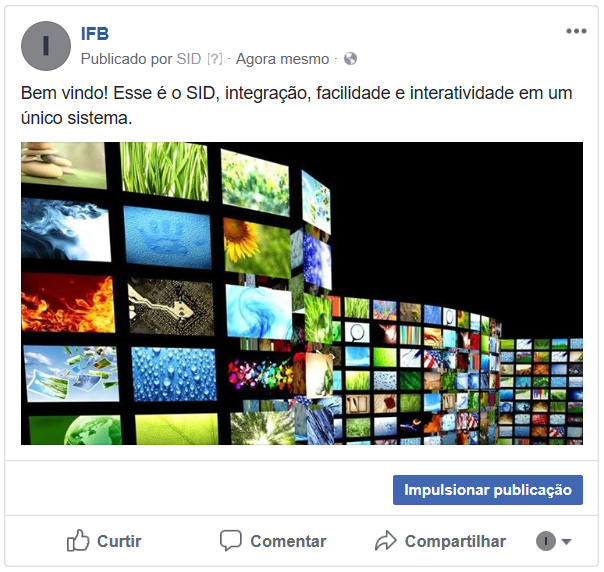
\includegraphics[scale=1]{figuras/imgfacebook1}
\caption{Divulgação enviada ao Facebook com auxílio do SID}
\label{fig:imgfacebook1}
\end{figure}


\subsection{Requisitar}
Usando o ID da foto é possível recuperar informações das arestas, que podem ser a URL, os comentários e as curtidas conforme o exemplo \ref{lst:requisicao8}. Esse recurso é utilizado para recuperar os mais diversos elementos que as permissões concedidas autorizam, entre os elementos recuperados estão o endereço da publicação, os comentários, curtidas e a imagem de perfil que serão apresentados respectivamente nos campos destinados ao QRCode e na coluna de comentários do módulo cliente.

\section{Possível solução para Implantação - Rapberry}
Desde a sua invenção em 1971, microprocessadores vem sendo usados no desenvolvimento dos mais variados tipos de eletrônicos ou outros equipamentos, substituindo até mesmo sistemas mecânicos. Algo que vai além de um simples software, os microprocessadores devem ser capazes controlar as ações de um dispositivo. \cite{rosenstark2007}

Para \cite{aristotelous2016}, o objetivo essencial de todos os tipos de empresa é a rentabilidade, podendo ela ser alcançada usando uma solução de baixo custo, boas tecnologias e com um preço atrativo. Teste do \cite{aristotelous2016} apresenta a possibilidade de se ter um servidor completamente funcional com sistema operacional Linux por um equipamento de 35\$, possibilitando a criação de um servidor, por exemplo de um repositório na nuvem com um baixo custo, flexibilidade e eficiência energética. 

Grandes servidores oferecem um melhor desempenho, entretanto, o baixo uso, a pouca eficiência energética ou até mesmo o pouco espaço podem limitar o uso desse tipo de equipamento. Nesse sentido, para \cite{cusick2014}, placas de circuito oferecem vantagens como o uso de pouco espaço, desempenho significante com baixo custo e consumo, além do suporte a diversas soluções de software oferecendo múltiplas opções de interface com uma variante do Linux. 
